\section{Electronics Hatch and Mounting}
\label{sec:electronics-hatch}

The Loon-E features a custom-designed electronics hatch located within the central cavity of the catamaran hull. The design prioritizes modularity, thermal management, and fail-safe water protection.

\subsection{Suspended Design Philosophy}
A key innovation of the Loon-E is the \textbf{suspended electronics mounting}. Unlike traditional designs where components are mounted to the floor of the hull, the Loon-E utilizes two electronics plates suspended from the hatch lid via aluminum brackets (see Figure \ref{fig:electronics-hatch}). 

This configuration provides a critical safety buffer: in the event of a minor hull breach or seal failure, incoming water will collect at the bottom of the hull cavity, keeping the sensitive microelectronics and high-voltage components dry in the air pocket above.

\subsection{Mechanical Construction and Waterproofing}
The hatch is secured using a series of latches that compress a rubber seal against the hull, creating a watertight environment.

\begin{itemize}
    \item \textbf{Mounting Plates:} The system utilizes two plates. For production, \textbf{aluminum} is preferred to act as a secondary heat sink for the Jetson Orin Nano and motor controllers. For rapid prototyping, \textbf{acrylic} plates are used to allow for easy drilling and repositioning of components.
    \item \textbf{Modularity:} The vertical stack design maximizes the available internal volume, allowing components to "overlap" at different heights. This ensures there is sufficient room for future sensor expansions or larger battery packs.
    \item \textbf{External Interfaces:} Connections to external sensors (ZED X camera) and thrusters are made via IP-rated waterproof connectors and watertight heat-shrink tubing to prevent ingress through the cable runs.
\end{itemize}

\begin{figure}[H]
    \centering
    % Image based on Technical Report Appendix C
    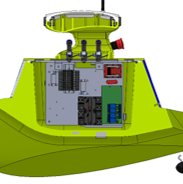
\includegraphics[width=0.8\textwidth]{images/Loon_E_Cross_Section.png}
    \caption{Cross-section of the Electronics Hatch showing suspended mounting (Ref: Technical Report Fig. 4)}
    \label{fig:hatch-assembly}
\end{figure}